% This file contains text to create bios for EnICS members and close collaborators

%%%%%%%%%%%%%%%%%%%%%%%%%%%%%%%%%%%%%%%%%%%%%%%%%%%%
%%%                  Faculty                     %%%
%%%%%%%%%%%%%%%%%%%%%%%%%%%%%%%%%%%%%%%%%%%%%%%%%%%%

%<*AdamTeman>
\begin{IEEEbiography}    [{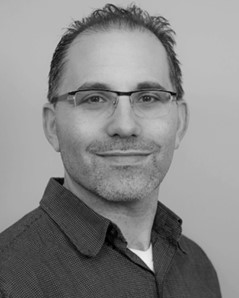
\includegraphics[width=1in,height=1.25in,clip,keepaspectratio]{./Bios/adam_teman.jpg}}]
    {Adam Teman} (M'14,SM'23) received the Ph.D. degree in electrical and computer engineering from Ben-Gurion University (BGU), Be’er Sheva, in 2014. He worked as a Design Engineer at Marvell Semiconductors, from 2006 to 2007. From 2014 to 2015, he was a Postdoctoral Researcher at the École Polytechnique Fédérale de Lausanne (EPFL), Switzerland, under a Swiss Government Excellence Scholarship. Since 2015, he has been with Bar-Ilan University, where he is an Associate Professor and the Co-Director of the Emerging Nanoscaled Integrated Circuits and Systems (EnICS) Laboratories. In 2021, he co-founded RAAAM Memory Technologies, where he is head of Product Development. He has authored over 115 scientific articles and holds 11 patents. His research interests include embedded memories, energy-efficient circuit design, hardware for artificial intelligence, open source processor platforms and accelerators, and methodologies for physical implementation. In 2020, he was awarded the Krill Prize for outstanding young researchers. 
\end{IEEEbiography}
%</AdamTeman>

%<*LeonidYavits>
\begin{IEEEbiography}[{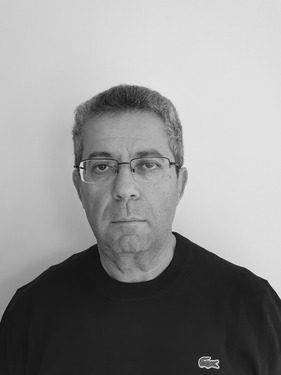
\includegraphics[angle=0,width=1in,height=1.25in,clip,keepaspectratio]{./Bios/leonid_yavits.jpg}}]{Leonid Yavits} 
    is with the Faculty of Engineering, Bar-Ilan University, Israel. He received his MSc and PhD degrees in electrical engineering from Technion, Israel. Leonid is a serial entrepreneur who was involved in co-founding and successful management (from a concept to M\&A) of several start-ups in the field of ASICs. His research interests include bioinformatics, domain specific accelerators, and processing in memory.
\end{IEEEbiography}
%</LeonidYavits>

%<*AlexFish>
\begin{IEEEbiography}    [{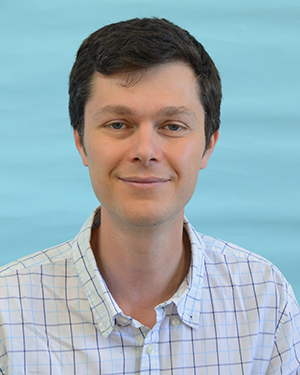
\includegraphics[width=1in,height=1.25in,clip,keepaspectratio]{./Bios/Alexander_Fish.png}}]
    {Alex Fish} (Member, IEEE) received the B.Sc. degree in Electrical Engineering from the Technion, Israel Institute of Technology, Haifa, Israel, in 1999. He completed his M.Sc. in 2002 and his Ph.D. (summa cum laude) in 2006, respectively, at Ben-Gurion University in Israel. He was a postdoctoral fellow in the ATIPS laboratory at the University of Calgary (Canada) from 2006-2008. In 2008 he joined the Ben-Gurion University in Israel, as a faculty member in the Electrical and Computer Engineering Department. There he founded the Low Power Circuits and Systems (LPC\&S) laboratory, specializing in low power circuits and systems. In July 2011 he was appointed as a head of the VLSI Systems Center at BGU. In October 2012 Prof. Fish joined the Bar-Ilan University, Faculty of Engineering as an Associate Professor and the head of the nanoelectronics track. In March 2015 he founded Emerging nanoscaled Integrated Circuits and Systems (ENICS) labs. Currently, he is a Full Professor and a co-director of the EnICS Impact Center. \\
    Prof. Fish’s research interests include power reduction methodologies for high speed digital and mixed signal VLSI chips, energy efficient SRAM and eDRAM memory arrays, CMOS image sensors and biomedical circuits, systems and applications, and cryogenic CMOS circuits. He has authored over 190 scientific papers in journals and conferences. He also submitted more than 30 patent applications of which 22 were granted. Prof. Fish has published three book chapters and two books as an editor. \\
    Prof. Fish founded and served as an Editor in Chief for the MDPI Journal of Low Power Electronics and Applications (JLPEA) from 2012 to 2018 and was an Associate Editor of IEEE various journals. Today he is an Associate Editor of IEEE Access Journal, Microelectronics Journal (Elsiever), and Integration, the VLSI journal (Elsiever). He also served as a program chair and chair of different tracks of various IEEE conferences. He was a co-organizer of many special sessions at IEEE conferences, including IEEE ISCAS, IEEE Sensors, and IEEEI conferences. Prof. Fish is a member of the Technical Committee of the European Solid-State Circuits Conference.  He is also a member of the VLSI Systems and Applications and Bio-medical Systems Technical Committees of IEEE Circuits and Systems Society.. 
\end{IEEEbiography}
%</AlexFish>

%<*YossieShor>
\begin{IEEEbiography}    [{\includegraphics[width=1in,height=1.25in,clip,keepaspectratio]{./Bios/yossie_shor.jpg}}]
    {Yossie Shor} (Senior Member, IEEE) PhD and MS in Electrical Engineering from Columbia University, 1993 and 1988 respectively. BA in Physics, Queens College, 1986. Prof. Shor has published more than 70 papers in refereed Journals and Conference Proceedings in the areas of Analog Circuit Design and Device Physics.  He holds over 50 issued patents and several pending patents. He is presently a Full Professor of Electrical Engineering at Bar Ilan University, Ramat Gan, Israel. From 2004-2015, he was at Intel Israel, as a Principal Engineer, and head of the Analog Team at Intel Yakum. Between 1999-2004, he worked at Saifun Semiconductor, Netanya, Israel, as a Staff Engineer where he established the analog activities for Flash and EEPROM NROM memories.  From 1994-1999, he was a Senior Analog Designer at Motorola Semiconductor, Israel, in the DSP Division.   From 1988-1994, he was a Senior Research Scientist at Kulite Semiconductor, NJ, USA, where he developed processes and devices for Silicon Carbide and Diamond Microsensors.  His present interests include Analog circuits, Switching and Linear Voltage Regulators, Sensors, PLLs and IO circuits, Microprocessors and Security. He was a member of the ISSCC Technical Program Committee (TPC) from 2014-2018, is a member of the TPC and Steering Committee of ESSCIRC, and is an Associate Editor for IEEE SSCL and IEEE Sensors Journal.  He has been a guest Associate Editor of JSSC and SSCL. For more information, see his personal website at http://www.eng.biu.ac.il/shorjos/ 
\end{IEEEbiography}
%</YossieShor>

%<*ItamarLevi>
\begin{IEEEbiography}[{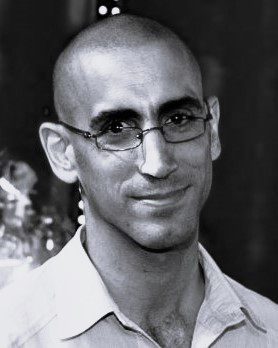
\includegraphics[width=1in,height=1.25in,clip,keepaspectratio]{Bios/ItamarLevi.jpg}}] {Itamar Levi} (Member, IEEE) 
    received his B.Sc. and M.Sc. degrees in Electrical and Computer Engineering as a part of a direct excellence student track from Ben-Gurion University in 2012 and 2013, respectively.
    He completed his Ph.D. at Bar-Ilan University in 2017.
    He was a research-associate in UCLouvain, Belgium until 2019 with the UCLouvains Crypto-Group and currently he is a Computer-Engineering Faculty member at Bar-Ilan University, in Ramat Gan, Israel. He is also a member of the Emerging Nanoscaled Circuits and Systems (EnICS) Labs at BIU. Dr. Levi’s current research interests are digital circuit design, embedded systems security, security evaluation analysis for cryptographic devices, side-channel and fault-injection countermeasures, and cryptographic implementations. He has (co-)authored over 60 journal articles and international conference papers and 7 patent applications. He co-authored a book called ``Dual-Mode-Logic: A New Paradigm for Digital IC Design'' and serves in various Technical Committees of IEEE CAS Society and Hardware Security journals and conferences.
\end{IEEEbiography}
%</ItamarLevi>

%<*OsnatKeren>
\begin{IEEEbiography}    [{\includegraphics[width=1in,height=1.25in,clip,keepaspectratio]{./Bios/osnat_keren.jpg}}]
    {Osnat Keren} (Member, IEEE) . 
\end{IEEEbiography}
%</OsnatKeren>



%%%%%%%%%%%%%%%%%%%%%%%%%%%%%%%%%%%%%%%%%%%%%%%%%%%%
%%%                  SoC                         %%%
%%%%%%%%%%%%%%%%%%%%%%%%%%%%%%%%%%%%%%%%%%%%%%%%%%%%
%<*YoavWeitzman>
\begin{IEEEbiography}[{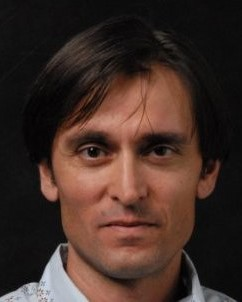
\includegraphics[width=1in,height=1.25in,clip,keepaspectratio]{./Bios/Yoav_Weizman.png}}] 
    {Yoav Weizman} received his Ph.D. degree in physics from Ben-Gurion University. He has over 20 years of experience in basic and applied research, development, and design. In 2000 he joined Freescale Semiconductor, Hertzelia, where he was involved in the development of tools and techniques for IC diagnostics and later became Product Analysis and Characterization Manager leading research activities in failure analysis, signal integrity and special IC diagnostics structures for yield enhancement and process tuning. Dr. Weizman joined Bar Ilan University at 2013 as research fellow and is involved since in numerous studies of IC reliability, circuit methods to mitigate HW tempering and eavesdropping. He also developed several unique approaches for PUF and RNG implementations which were implemented successfully in test chips. Dr. Weizman published over 50 papers and 16 patents.
\end{IEEEbiography}
%</YoavWeitzman>

%<*YonatanShoshan>
\begin{IEEEbiography}    [{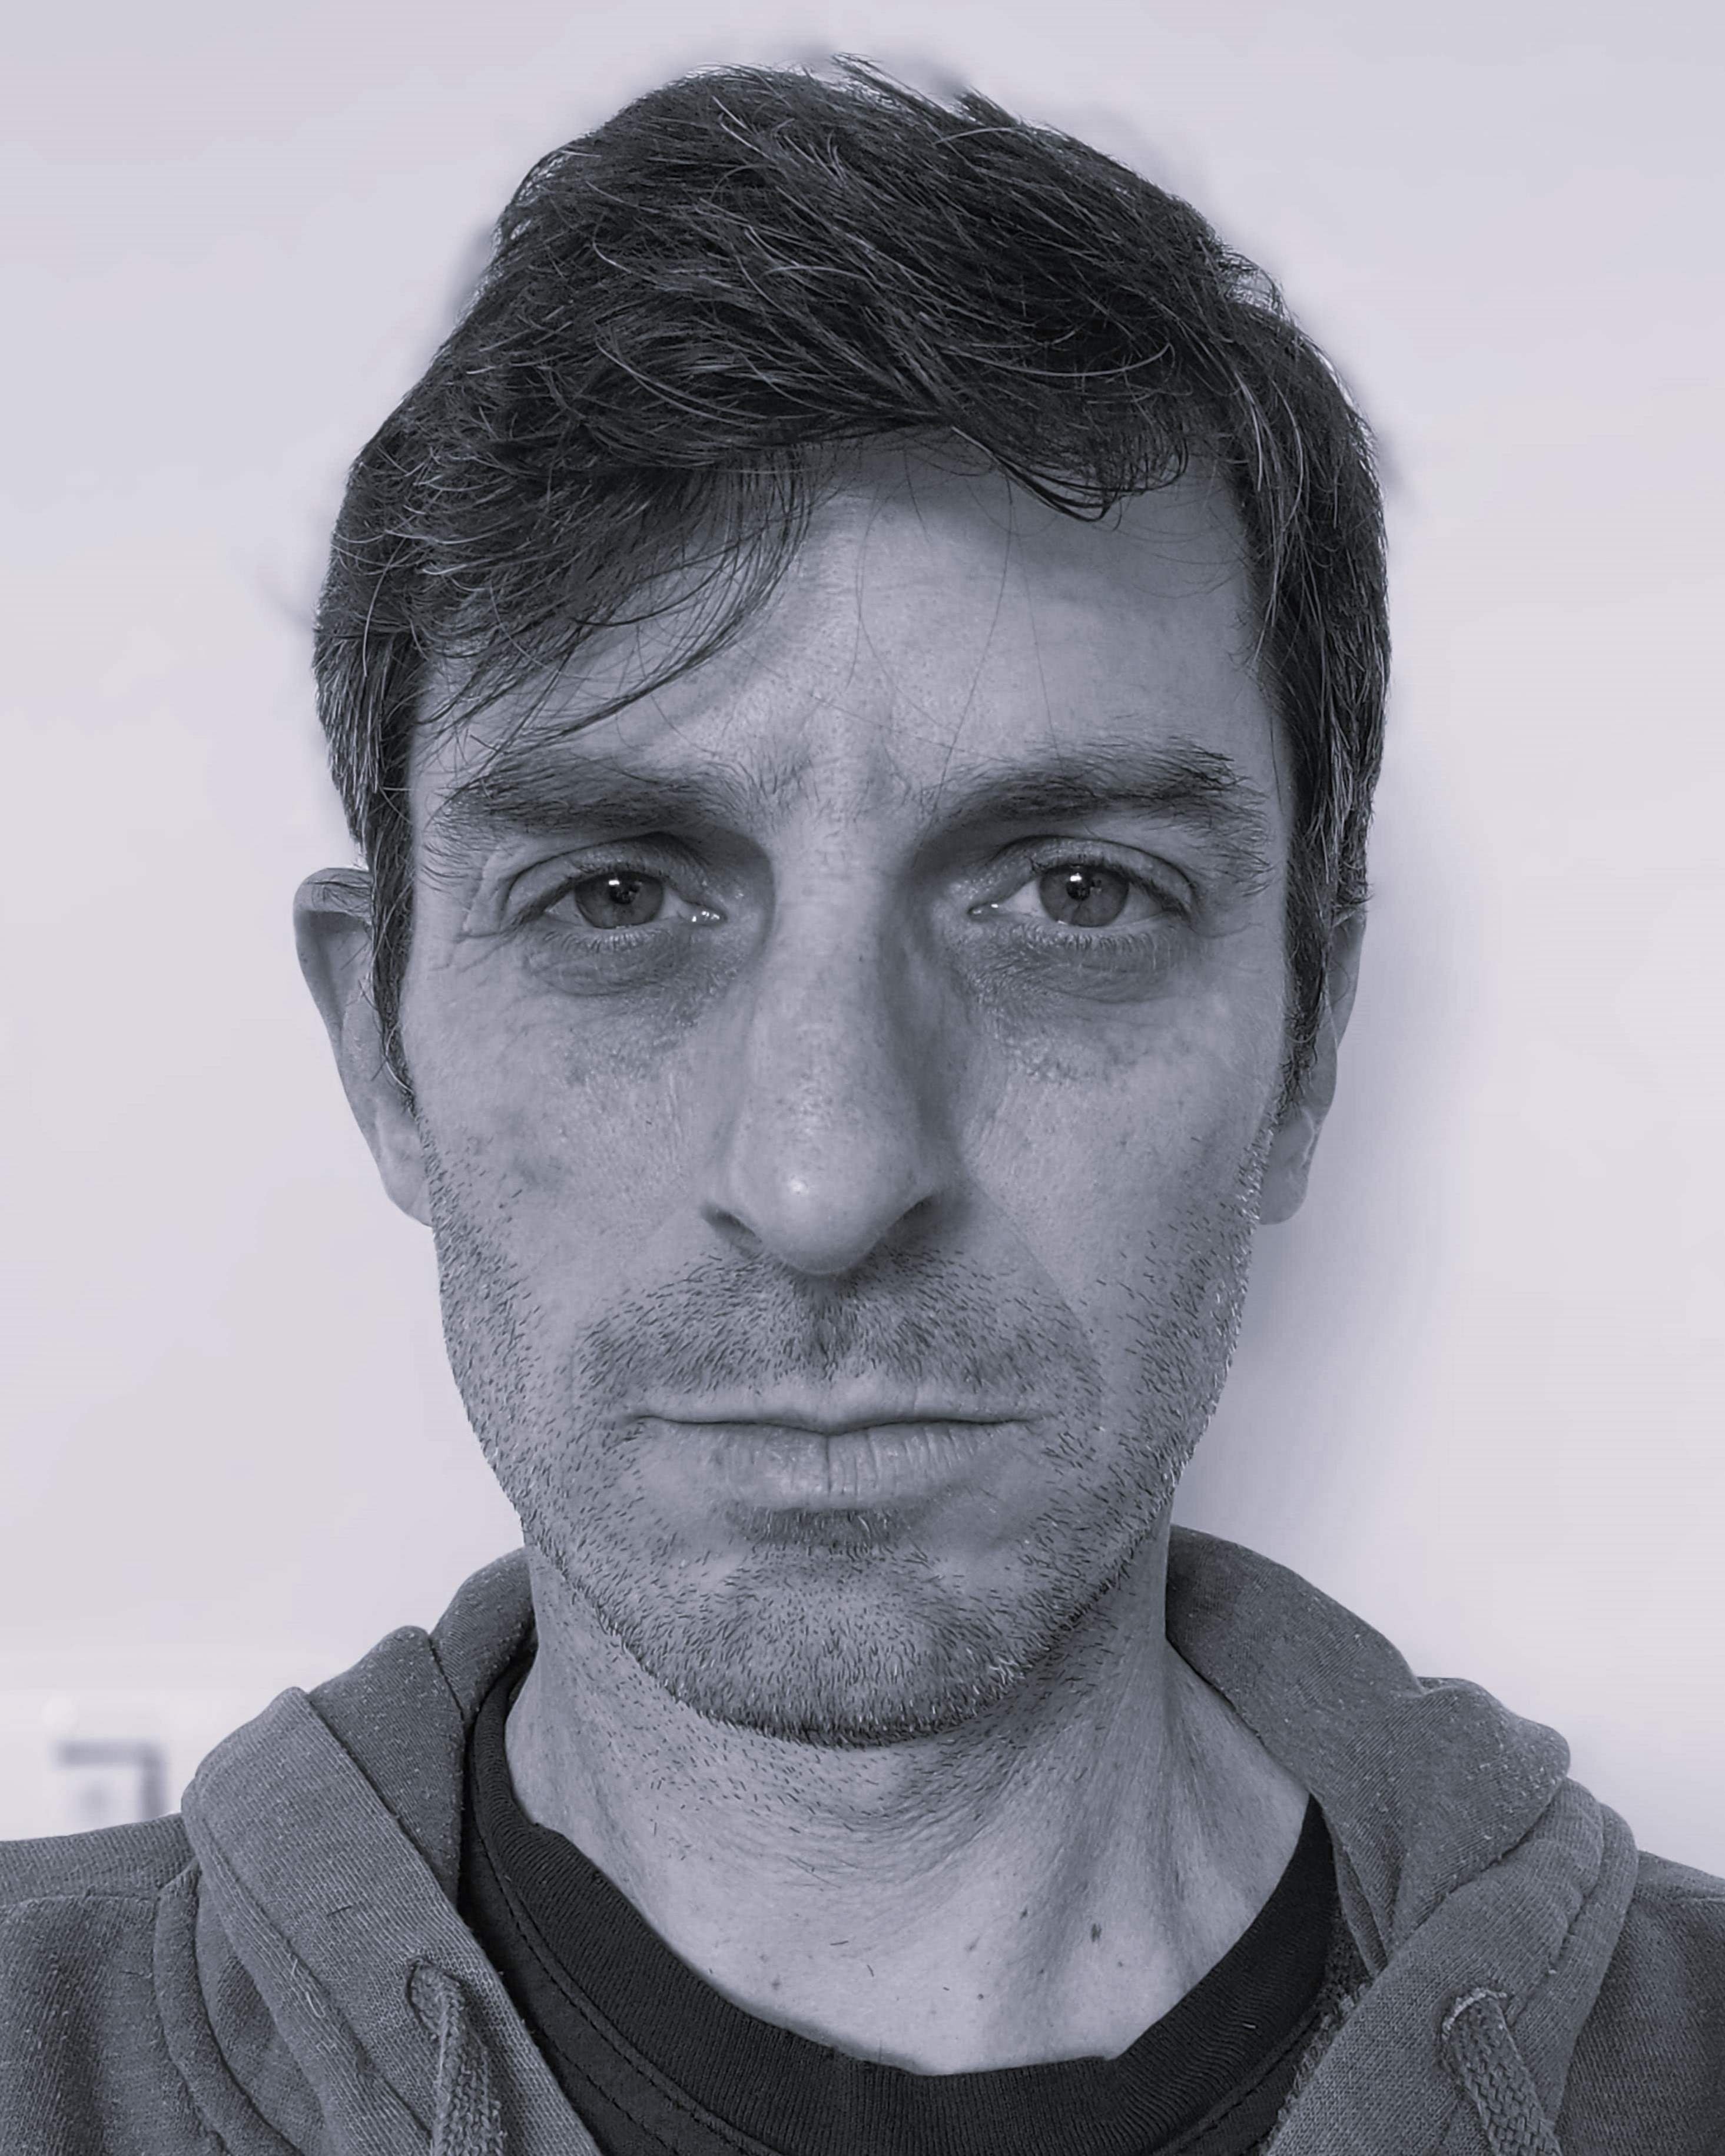
\includegraphics[width=1in,height=1.25in,clip,keepaspectratio]{./Bios/yonatan_shoshan.jpg}}]
    {Yonatan Shoshan} received the B.Sc. degree in electrical and computer engineering from Ben Gurion University, Beer Sheba, Israel, in 2006 and the M.Sc. degree in electrical and computer engineering from University of Calgary, Alberta, Canada, in 2009. He is currently pursuing the Ph.D. degree in electrical and computer engineering at Bar Ilan University, Israel. From 2009 to 2015, he was a digital design engineer in the field of wireless and wired communication with Siverge Networks and Texas Instruments, Israel. His research interests include digital circuits and embedded processing and SoC design, as well as circuits and systems for quantum computers controllers and error correction decoders. 
\end{IEEEbiography}
%</YonatanShoshan>

%<*YehudaRudin>
\begin{IEEEbiography}    [{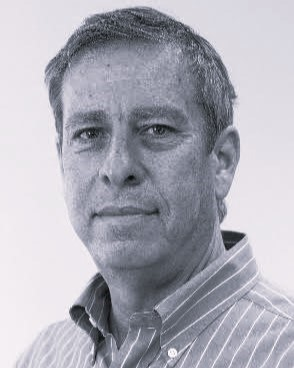
\includegraphics[width=1in,height=1.25in,clip,keepaspectratio]{./Bios/yehuda_rudin.jpg}}]
    {Yehuda Rudin} received the BSc degree in Computer Engineering from the Technion, Haifa, in 1985 and the MSc  degree in Electrical Engineering from Bar-Ilan University, Ramat-Gan, in 2022. He worked at Motorola Semiconductor and later Freescale Semiconductor from 1987 to 2016 in various senior R\&D positions. He became a Freescale Fellow in 2012 and was the General Manager of the Freescale Design Center in Israel from 2013 to 2016. Since 2016, he has been with Bar-Ilan University, where he is a General Manager of the Emerging Nanoscaled Integrated Circuits and Systems (EnICS) Laboratories. Yehuda is currently a Ph.D. student in the Faculty of Engineering, Bar-Ilan University.
\end{IEEEbiography}
%</YehudaRudin>


%<*UdiKra>
\begin{IEEEbiography}    [{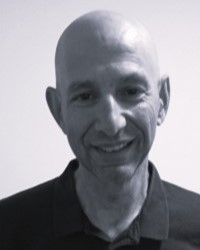
\includegraphics[width=1in,height=1.25in,clip,keepaspectratio]{./Bios/udi_kra.jpg}}]
    {Yehuda (Udi) Kra} received the B.Sc. degree in electrical engineering from the Technion, Israel Institute of Technology in 1985, and the MSc degree from Bar-Ilan University  in 2022. He has over 35 years of experience in design, research, innovation, entrepreneurship, and management in the semiconductor industry, specializing optimized IC solutions.  In 2018  he  joined the Emerging Nanoscaled Integrated Circuits and Systems (EnICS) Research Center at Bar-Ilan University as the Chief Architect of the RISC-V embedded processor project as part of the Israeli Innovation Authority GenPro Consortium. Currently Kra is pursuing his PhD degree focusing on advanced hardware-accelerated Machine-Learning computation platforms.
\end{IEEEbiography}
%</UdiKra>

%%%%%%%%%%%%%%%%%%%%%%%%%%%%%%%%%%%%%%%%%%%%%%%%%%%%
%%%                  UNICAL                      %%%
%%%%%%%%%%%%%%%%%%%%%%%%%%%%%%%%%%%%%%%%%%%%%%%%%%%%
%<*EstebanGarzon>
\begin{IEEEbiography}[{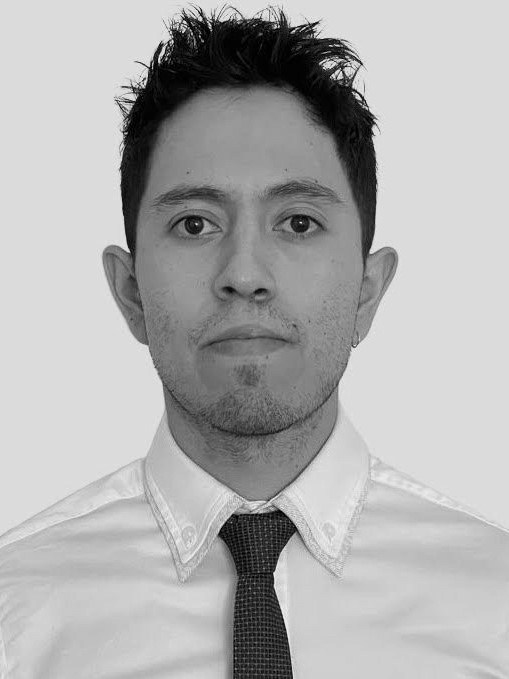
\includegraphics[width=1in,height=1.25in,clip,keepaspectratio]{./Bios/esteban_garzon.jpg}}]{Esteban~Garzón}
    (Member, IEEE) received the Ph.D. degree in electronics engineering from the University of Calabria (UNICAL), Italy, in 2022. He is currently a Postdoctoral Researcher at the Department of Computer Engineering, Modeling, Electronics and Systems Engineering, UNICAL. He has coauthored more than 30 scientific papers in international journals and conferences, and has participated in several IC tapeouts. His research interests include domain-specific hardware accelerators, and electronics/spintronics, cryogenic memories, and standard and emerging technologies for logic, memory, and low-power applications. 
\end{IEEEbiography}
%</EstebanGarzon>

%<*MarcoLanuzza>
\begin{IEEEbiography}[{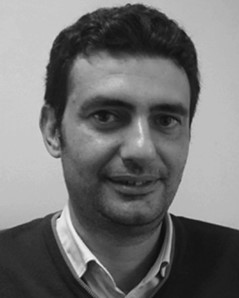
\includegraphics[width=1in,height=1.25in,clip,keepaspectratio]{./Bios/marco_lanuzza.jpg}}]{Marco Lanuzza}
    (Senior Member, IEEE) received the Ph.D. degree in electronic engineering from the Mediterranea University of Reggio Calabria, Reggio Calabria, Italy, in 2005. Since 2006, he has been with the University of Calabria, Rende, Italy, where he is currently an Associate Professor. He has authored over 120 publications in international journals and conference proceedings. His recent research interests include the design of ultralow voltage circuits and systems, the development of efficient models and methodologies for leakage- and variability-aware designs, and the design of digital and analog circuits in emerging technologies. Prof. M. Lanuzza is an Associate Editor of Integration, the VLSI Journal.
\end{IEEEbiography}
%</MarcoLanuzza>

